\documentclass{article}%
\usepackage[T1]{fontenc}%
\usepackage[utf8]{inputenc}%
\usepackage{lmodern}%
\usepackage{textcomp}%
\usepackage{lastpage}%
\usepackage{authblk}%
\usepackage{graphicx}%
%
\title{A SUMOylation{-}defective MITF germline mutation predisposes to melanoma and renal carcinoma}%
\author{Tiffany Kim}%
\affil{Department of Cardiology, Zhongda Hospital, Medical School of Southeast University, Nanjing, Jiangsu, China}%
\date{01{-}01{-}2014}%
%
\begin{document}%
\normalsize%
\maketitle%
\section{Abstract}%
\label{sec:Abstract}%
DUSP1 is a Novel Target for Enhancing Pancreatic Cancer Cell Sensitivity to Gemcitabine\newline%
SAN DIEGO {-} Novo Nordisk, the leading life science company dedicated to the discovery and development of therapeutic compounds which lead to the prevention and treatment of cancer, announced today that it has entered into a Biologics License Agreement (BLA) with NDS Pharmaceuticals to utilize an Agonist Cancer Cell Compound to develop drug candidates.\newline%
Blaisdell Diagnostics, Inc. and RADIANT are the exclusive licensing partners of DUSP1 in the U.S.\newline%
The DO{-}1929 Agonist Cancer Cell Compound was discovered by DUSP1 researchers who successfully brought two previous compounds to market. Now based at SMDC{-}The Roswell Park Cancer Institute, the DUSP1 clinical development program will use two DUSP1 inhibitors to advance its first program.\newline%
John Stewart, M.D., Executive Vice President and Chief Medical Officer, San Diego State University, said: Although DUSP1 has been fully studied in combination with gemcitabine in pancreatic cancer patients, we have not yet demonstrated a potent JAK4 affinity or impact on the JAK pathway. With this in mind, the prospect of using DUSP1 to actively enhance JAK4 is extremely promising, so we have selected a novel JAK4 inhibitor. Together, DUSP1 and JAK4 have been shown to target the metabolic mechanism at the molecular level and in so doing enable the blocking of several chemotherapeutic pathways including gemcitabine, which is used for the prevention and treatment of cancer, but due to its potency and cost it is ultimately no longer commercially viable for cancer patients.\newline%
Additional partnering details will be released at a later date.

%
\subsection{Image Analysis}%
\label{subsec:ImageAnalysis}%


\begin{figure}[h!]%
\centering%
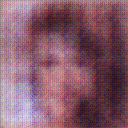
\includegraphics[width=150px]{500_fake_images/samples_5_302.png}%
\caption{A Close Up Of A Cat In A Window}%
\end{figure}

%
\end{document}